\documentclass{article}[letter,10pt]
\usepackage{biblatex}[encoding=utf8,backend=biber]
\addbibresource{turtles.bib}
\AtBeginBibliography{\setcounter{maxnames}{5}\setcounter{minnames}{5}}
\usepackage{geometry}[tmargin=1in,bmargin=1.5in,lmargin=1in,rmargin=1in]
\usepackage{longtable}
\pagenumbering{gobble}
\usepackage{chngcntr}
\counterwithin{table}{subsection}
\usepackage{subcaption}
\usepackage{tabularx}
\usepackage{booktabs}
\usepackage{float}
\usepackage{pgfplots}
\usepackage{tikz}
\usetikzlibrary{patterns}
\pgfplotsset{
  tick label style={font=\footnotesize},
  label style={font=\small},
  legend style={font=\small},
  compat=newest
}

\title{Release the TURTLES\\
  \large{A Pure Tcl Interface to Dynamic Proc Tracing}}
\author{
  Michael Yantosca\\
  FlightAware \\
  michael.yantosca@flightaware.com
}

\begin{document}

\maketitle

\begin{abstract}
  Proper dynamic program analysis requires solid collection of call frequency,
  relationships, and timing. Typically, this is achieved with a suite of
  language-centric tools, e.g., valgrind (C/C++), the GHC profiling subsystem
  (Haskell). Tcl appears to lack similar tools or at least requires significant
  language extensions to meet this need. Consequently, this work introduces
  the Tcl Universal Recursive Trace Log Execution Scrutinizer (TURTLES), a
  simple proc tracing interface that yields easily aggregated and analyzed
  call records. By adhering to pure Tcl, the endeavor provides an enlightening
  étude in the pain points of developing such tooling in the language.
\end{abstract}

\section{Introduction}{
  \paragraph{}{
    The TURTLES project began as a small task meant to investigate the
    relationship between different procs within the Tcl repositories comprising
    the FlightAware codebase, particularly for the Multi-Machine HyperFeed (MMHF)
    project. The results of the analysis would be leveraged to inform
    refactoring efforts to improve the performance of the target program.
    Inspired by callgrind\autocite{callgrind} and the GHC profiling
    subsystem\autocite{ghcprof}, the TURTLES project aimed to capture not
    only the call-graph relationships but also performance metrics so that
    users of the library could consolidate correlated calls into logical
    modules as well as pinpoint execution hotspots.
  }
  \paragraph{}{
    Some initial investigation was made into extant facilities within
    the Tcl base or community packages that might achieve this purpose.
    Shannon Noe suggested cmdtrace\autocite{tcl::cmdtrace} and
    disassemble\autocite{tcl::disassemble} as potential candidates.
    After reviewing the documentation, the disassembler appeared to
    be worth investigating as a tool for static analysis in future work.
    To determine the suitability of cmdtrace for dynamic analysis, some dry
    runs were executed on toy programs with cmdtrace turned on. The resulting
    output was verbose and would require extra parsing to convert into
    a usable format. The parsing work was not necessarily prohibitive, but
    complex programs like MMHF could potentially generate unmanageable amounts
    of data, and so it was deemed that a more space-sensitive approach was
    required.  To this end, constraints were placed on the scope of the TURTLES
    project to only examine the immediate caller/callee relationship and provide
    execution timings inclusive of the total time spent both in the callee and
    in the callee's subcalls.
  }
  \paragraph{}{
    The TURTLES project also served as an introductory étude in Tcl introspection.
    As a neophyte in the language, working on the TURTLES project offered an
    accelerated course in namespace management and execution semantics. Pursuing
    a pure Tcl approach forced careful consideration of the costs incurred by
    the profiling overhead and exposed some pitfalls in Tcl that might
    be improved in future revisions of the language to make it more accessible
    and productive for both novice and experienced developers.
  }
  \paragraph{}{
    In order to maximize portability, one tacit goal of the TURTLES is to have
    minimal dependencies on other packages. The list of required packages is
    given as follows:
    \begin{itemize}
    \item{Tcl 8.5\autocite{tcl::85} or 8.6\autocite{tcl::86}}
    \item{Tclx\autocite{tcl::Tclx}}
    \item{Thread\autocite{tcl::Thread}}
    \item{cmdline\autocite{tcl::cmdline}}
    \item{platform\autocite{tcl::platform}}
    \item{sqlite3\autocite{tcl::sqlite3}}
    \item{tcltest\autocite{tcl::tcltest}}
    \end{itemize}
    Building the project requires GNU make or a compatible make utility.
    Code documentation can be generated by doxygen, but installation does
    not require it. The project repository README provides instructions
    on building and installing the TURTLES project, as well as instructions
    for use within a given user-defined program. Some aspects of usage
    will also be covered in the Design and Implementation sections of
    this report.
  }
  \paragraph{}{
    The remainder of this report is organized in the following manner.
    The Design section covers the abstract design decisions and data flow
    for the TURTLES project. The Implementation section expounds on the
    Design section with specific details about how the design was realized.
    The Experiments section exhibits the results of employing the TURTLES
    project on both toy examples and on the larger MMHF project.
    In the Conclusions section, the experimental results and the development cycle
    of the TURTLES project are evaluated along with some aspects of the Tcl learning curve.
    Finally, in the Future Work section, some avenues for ongoing research
    are considered in light of the aforementioned conclusions with the goal of
    improving the TURTLES project so as to encourage adoption and enhance
    the set of available tools for Tcl development.
  }
}

\section{Design}{
  A few guiding principles informed the design of the TURTLES project, namely
  minimization of overhead, correctness of collection, ease of use, and legibility
  of results. For simplicity, the call records do not attempt to store information
  for complete traces through the full call stack but rather capture the immediate
  caller-callee relationship.

  \subsection{Initialization}{
    Starting data collection is achieved by a designated proc which sets up
    the necessary ephemeral and final storage for call records per arguments
    supplied by the user. A trace handler is added to the \texttt{proc} command on exit
    to bootstrap the assignment of trace handlers for entry and exit to every
    proc defined thereafter.

    For best results, it is recommended to make the initialization call as early
    as possible to capture the greatest number of proc definitions. Currently,
    the TURTLES project does not support retroactively adding proc handlers
    to procs already defined.

  }
  \subsection{Collection}{
    The entry and exit handlers capture the times of entry and exit into and out of
    the covered proc and record this in the form of a call point record. The caller
    and callee information in each call point record is normalized out to a collection
    of unique proc definition records.

    \paragraph{Proc Definition}{
      Each proc defined after data collection starts is stored in a proc definition
      record. This record is a triple of the proc name, a unique integral identifier,
      and the time of definition. The proc name is the unaliased, fully-qualified
      name of the proc, and the integral identifier is a hash of this value.
      The time of definition is canonically represented in UNIX epoch microseconds.
    }
    \paragraph{Call Point}{
      Each call made is recorded in the form of a call point record. This record
      is a quintuple consisting of a caller ID, callee ID, trace ID, time of
      entry, and time of exit. The caller and callee IDs correspond to unique
      integral identifiers in the set of proc definition records. The trace ID is a
      unique identifier for distinguishing separate calls with the same caller
      and callee and is calculated deterministically. Time of entry and exit are
      canonically represented in UNIX epoch microseconds.
    }
    \paragraph{Persistence}{
      Persistence of call records is handled either directly or in a staged fashion
      depending on the arguments supplied by the user. In direct mode, the call
      records are captured and stored immediately in the final storage. This has
      the benefit of retaining the most information in case execution is interrupted
      but at the cost of speed. In staged mode, the call records are captured and
      stored in ephemeral storage while a background task or thread periodically
      transfers unfinalized records in bulk to the final persistent storage. The
      immediate processing cost of each call record is reduced, but the risk of
      greater overall loss in cases of interruption is increased.
    }
  }
  \subsection{Finalization}{
    Ending data collection is achieved by a designated proc which disables
    all the relevant trace handlers along with the handler on the \texttt{proc} command.
    If collection was operating in staged mode, the ephemeral storage is flushed
    to the final storage.
  }
  \subsection{Analysis}{
    For post-hoc analysis, a clustering tool is provided to construct a call graph
    whose edges are the immediate caller-callee pairings and nodes are individual
    procs. The edge weights are defined as the number of invocations of the callee
    by the caller.

    In anticipation of a highly-connected graph with many nodes, initial attempts
    to realize the clustering tool employed the Gallagher-Humblet-Spira (GHS) distributed
    minimum spanning tree algorithm\autocite[102-106]{DNA}. Development of a $k$-machine
    model\autocite[129-133]{DNA} using Tcl threads as the individual machines was started but ultimately
    abandoned due to low development velocity. In its place, a simple breadth-first
    flooding approach\autocite[55-58]{DNA} was adopted and found to be sufficient to the task.

    The call records themselves are stored in a format that is searchable and aggregable
    via standard SQL statements. This provides the developer with an expressive foundation
    for data analysis and visualization which has long enjoyed wide adoption with a
    minimal learning curve.
  }
}

\section{Implementation}{
  As a pure Tcl implementation, the TURTLES project relies heavily on the
  introspection facilities in the language, particularly trace handlers.
  This section examines some of the implementation details and provides
  justification for the decisions made.

  \subsection{Integration}{
    For most users, installing the library in the Tcl search path and placing
    the directive \texttt{package require turtles} inside the target program's source
    should suffice to enable usage of the library. The project \texttt{README.md} contains
    instructions on installation, as well as commencement and termination of data
    collection in the ostensibly common case. The particulars of usage and data collection
    are covered in following subsections.
  }

  \subsection{Parameterization}{
    A set of command-line arguments are used to parameterize the call record collection at runtime.
    The command-line parameters themselves are bracketed by the literals \texttt{+TURTLES} and \texttt{-TURTLES}
    to distiguish TURTLES parameters from program arguments.
    The arguments to TURTLES may be interspersed anywhere in the command line provided that
    they are appropriately bracketed.

    During initialization, \texttt{::turtles::options::consume} takes the name reference of an
    \texttt{argv}-style string and destructively consumes the TURTLES parameters from that variable.
    Therefore, it is strongly recommended to place the initialization call to
    \texttt{::turtles::release\_the\_turtles} as close to the main entry point of the target program
    as possible, preferably before the program's own command-line argument parsing.

    Extensive instructions on command-line usage is available in the doxygen code documentation
    for \texttt{turtles.tcl}, but the gist of each option is replicated here for the convenience of the reader.

    \subsubsection{\texttt{-enabled}}{
      The TURTLES library remains dormant unless explicitly enabled. This enables programs to
      be instrumented with the TURTLES library without having to require boolean debug flags
      in the source. If the flag is not set at the command-line, collection will not happen
      since the trace handlers and persistence mechanisms will not be created at all, avoiding
      even idle overhead.
    }
    \subsubsection{\texttt{-commitMode (direct|staged) [-intervalMillis <ms>] [-scheduleMode (ev|mt)]}}{
      As mentioned in the Design section, the TURTLES library can persist call records
      either directly to final storage or indirectly to ephemeral storage which is
      persisted to final storage at regular intervals. For the indirect staged mode,
      the interval is specified in milliseconds as an argument to the \texttt{-intervalMillis}
      command-line switch. For direct mode, the \texttt{-intervalMillis} argument may be
      omitted. The default mode is \texttt{staged}, and the default finalization
      interval is \texttt{30000}, or 30s.

      Persistence is implemented through the use of SQLite databases. Ephemeral
      storage is an in-memory database, while final storage is a database file
      that is attached to the in-memory database in staged mode and immediately
      updated in direct mode.

      The \texttt{-scheduleMode} option indicates the method of dispath for the periodic
      finalization in staged commit mode. Under multithreaded mode, specified by \texttt{mt},
      the TURTLES library launches two separate Tcl threads, i.e., a recorder and a scheduler.
      The recorder handles all call record storage updates sequentially according to its thread
      snippet message queue including finalization operations. The scheduler periodically sends
      finalizing snippets to be processed by the recorder according to the configured interval.
      Under event-loop mode, specified by \texttt{ev}, the TURTLES library launches a self-recurring
      after job into the main Tcl event loop. This mode assumes that the event loop is entered
      subsequently after TURTLES initialization.
    }
    \subsubsection{\texttt{-dbPath <directory> -dbPrefix <string>}}{
      The \texttt{-dbPath} option specifies the directory path for the SQLite database serving
      as final storage. The actual database filename is specified by convention
      informed by the \texttt{-dbPrefix} option. The full filepath is
      determined as \texttt{<dbPath>/<dbPrefix>-<pid>.db} where \texttt{<pid>}
      is the operating system process ID of the program. By default, this will
      yield the filename \texttt{./turtles-<pid>.db}, i.e., \texttt{turtles-<pid>.db}
      in the current working directory during program execution. The path is canonicalized
      to an absolute path by the helper \texttt{::turtles::persistence::base::get\_db\_filename}.
    }
    \subsubsection{\texttt{-debug}}{
      Including the \texttt{-debug} flag in the TURTLES options turns on verbose logging
      of call record collection to \texttt{stderr}. This is useful during development to
      ensure calls are appropriately recorded but is not recommended for production runs.
    }
  }

  \subsection{Initialization}{
    Commencement of record collection is effected through calling \texttt{::turtles::release\_the\_turtles}
    with the \texttt{argv}-style command-line argument string reference.

    \subsubsection{Call Record Persistence}{
      Based on the parameters provided by the user, the TURTLES library opens the SQLite databases that
      serve as the requisite final and ephemeral call record storage.
    }
    \subsubsection{Trace Handlers}{
      A bootstrapping trace handler is attached to the \texttt{execution leave} event of the \texttt{proc} command.
      This handler has to determine the fully-qualified original name of the defined proc and
      add a handler each to the defined proc's \texttt{execution enter} and \texttt{execution leave} events,
      so it must be done post-definition so the two handlers can attach without an error.

      Additionally, the Tclx package is loaded and its version of the \texttt{fork} command is instrumented
      with handlers on \texttt{execution enter} and \texttt{execution leave}. This permits for
      some mitigation in case of process forking, which was a requirement of the MMHF program that
      engendered this experiment.
    }
  }

  \subsection{Collection}{
    \subsubsection{Deterministic Identification}{
      \paragraph{Proc ID}{
        The original name of each proc was hashed to an integral value using a Rabin-Karp rolling hash\autocite{univhash}.
        The mapping outputs in the range $[0, M_8]$, where $M_8$ is the 8th Mersenne prime, or $2^{31}-1$.
        Every caller and callee proc defined by the \texttt{proc} command has an entry created in the proc
        table of the output DB.
      }
      \paragraph{Trace ID}{
        Because the enter and leave handlers are defined separately, there needs to be a way to communicate
        between the handlers to ensure that the entry and exit of a specific call point are properly associated.
        This was the impetus for adding the trace id to the call point record. In the first implementation,
        each trace ID was an integer list hash of the following values: the caller ID, the proc ID, and the
        proc entry microsecond timestamp. Initially, a stack was used whereby the enter handler would push
        onto the stack and the leave handler would pop it off under the assumption of single-threaded execution.

        However, this did not account for yielding and other vagaries of the Tcl event loop, and it was
        observed that the trace IDs would not match up frequently in testing with non-trivial programs.
        To protect against this, a deterministic scheme was used so that the trace ID was computed
        as the integer list hash of the thread ID, stack level, caller ID, source line, and called ID.
        This had the additional benefit of saving the memory required for the stack at the cost of extra compute time.
        The stack level and source line were included in consideration of cases where a caller calls the callee
        numerous times in its body. The multi-threaded case has not been tested since it requires an
        initialization of TURTLES in each thread, and it is expected bugs will surface under those conditions,
        especially with respect to contention for the call record final storage.
      }
    }

    \subsubsection{Enter Handler}{
      The proc enter handler records its own computation start time, computes the requisite hashes for the call record,
      records a proc start time, and dispatches a snippet containing the provisional record to the persistence mechanism.
      The only information missing is the call point completion time, which is supplied by the leave handler.
      The proc enter handler records its computation stop time and dispatches a record of its own work out-of-band
      so as to prevent infinite recursion on proc entry.
    }

    \subsubsection{Leave Handler}{
      The leave handler first captures the proc computation end time. It then computes the requisite hashes and
      dispatches a snippet containing the partial record to the persistence mechanism. Like the proc enter handler,
      it keeps its own record of computation time that it sends out-of-band.
    }
    \subsubsection{Call Record Persistence}{
      Under the multi-threaded scheduling mode, the recorder thread receives snippet messages to execute.
      Call record messages come from the enter and leave handlers associated with the defined procs
      whether for the procs under observation or the handlers' own out-of-band execution metrics.
      For the staged case, a scheduler thread periodically sends snippets instructing the recorder to
      flush unfinalized call records from ephemeral to final storage.

      Under the event-loop scheduling mode, the scheduler is implemented as a self-recurring proc
      availing itself of Tcl's \texttt{after} mechanism. This requires the main program to enter the
      event loop at some point in time. Call records are immediately written to ephemeral storage
      in staged commit mode and final storage in direct commit mode.

      \paragraph{Fork Safety}{
        The MMHF program operates by performing some initialization and then forking multiple children of itself
        across which the stream processing load is balanced. Most of the procs to be instrumented are defined
        prior to the fork. In order to enable the TURTLES library to cross the fork boundary, the aforementioned
        enter handler on \texttt{Tclx::fork} finalizes whatever call records have been incurred during execution,
        shuts down the recorder and scheduler threads or event loop jobs, and closes the fork parent's final storage.

        The trace handlers as occupants of memory remain after the fork, and so the leave handler on \texttt{Tclx::fork}
        determines the fork child's process ID as well as the parent's for use in reconstructing the call record storage.
        The parent SQLite database is copied to a new child database, and since both databases are deterministically
        named by a convention that includes the process ID, conflicts should be minimized. Both children and parent
        reload their databases post-fork and restart the recorder and scheduler workers as applicable.

        There is a small window for lacunae in the call record history at the time of fork, but this is deemed
        an acceptable loss in light of the benefit that the implicit fork safety provides. Every child should have
        roughly the same information as the parent and its siblings pre-fork, subject to spawn order. This adheres
        to the copy semantics of forking at least by reasonable approximation if not exactly.

        Note that for long running programs, there is a potential for conflict if the parent process periodically
        refreshes the children and the operating system crosses the max PID boundary. In this case, a child may open
        a database that previously belonged to another child from the past. This is not a problem so long as there
        is a parent-child or sibling relationship between the processes that share the PID. The uniqueness of the
        trace ID for each call record is determined by both time (epoch execution microsecond stamps) and space
        (thread ID, call stack). This should make post-hoc merging of all the associated SQLite databases trivial
        provided that the merge ignores conflicts, which most likely will arise in most use cases from pre-fork records and the
        negligible probability of hash collision. Simultaneous runs of separate
        programs instrumented by TURTLES without specifying a unique database filename prefix per program
        will yield undesirable results.
      }
      \paragraph{Thread Safety}{
        Because the Tcl threading model defines a separate Tcl interpreter per thread, capturing call records
        in a multi-threaded scenario requires initialization at the start of each participating thread.
        This is not presently recommended since the behavior is untested, and as was previously alluded, it will
        probably result in contention for the call record database and possibly deadlock.

        The snippet message model used here incurs a substantial amount of overhead and requires that call record information
        be fully evaluated to literals since the threads do not share state. Thread state variables (TSVs) were
        eschewed to avoid the complexity of locking and state maintenance in favor of a stateless message-passing scheme.
      }
    }
  }

  \subsection{Finalization}{
    Finalization of call record storage is a simple process. Since SQLite permits attaching extraneous databases
    for information transfer, the finalization is done as a bulk insert query from ephemeral to final storage.
    Upon entry into the finalization procedure, the current clock is memoized and all records with non-null exit
    timestamps prior to the memoized cutoff are moved into final storage and deleted from ephemeral storage.
    The ephemeral storage has no need to maintain completed call records for update, and so this keeps the ephemeral
    storage size from growing without bound and improves the speed of update queries since there are fewer records
    to search.

    When the finalization procedure \texttt{::turtles::capture\_the\_turtles} is invoked,
    the applicable recorder and scheduler workers are stopped, and a final query moving call records
    from ephemeral storage to final storage is executed, including all records regardless of whether they had
    finished execution or not by the time the collection was ended.
  }

  \subsection{Analysis}{
    Considering the original ticket that spawned this project suggested the Highly Connected Subgraphs (HCS) algorithm\autocite{HCS}
    for clustering calls by connectivity, it should have been apparent \emph{ab initio} that attempting to implement
    GHS in a $k$-machine model implemented in Tcl threads was a bit overkill. Constructing a Tcl thread $k$-machine
    model would be an interesting project in its own right but falls outside the scope of this work. The work-in-progress
    is left in the repository under the \texttt{::turtles::bale} and \texttt{::turtles::kmm} namespaces as an
    interesting if incomplete attempt at realizing the algorithm. The implementation borrows heavily from work
    done by the author\autocite{ghscoco} on a connected components project using MPI\autocites{mpi}{openmpi} as the underlying framework.

    The BFS flooding implementation is implemented in the standalone \texttt{cluster.tcl} program, which loads
    the call records from the SQLite database that served as final storage for a given run into a weighted graph
    implemented as a nested set of dictionaries. The weights in the graph are the number of calls made by a caller
    to its callee.

    A \texttt{-cutoff} command-line argument informs the program to ignore edges below a certain weight.
    An \texttt{-undirected} flag informs the program to consider the edge between caller and callee in both
    directions. By default, it only adds edges radiating from the caller. In many cases, radiating edges from
    the callee as well will speciously connect procs by common primitives like \texttt{clock}. While this is useful
    for identifying procs that may need to be placed in a common base package, it may not provide much benefit
    for classifying procs according to behavior or subject.

    The level of verbosity in output may be varied at the command line, as well. By providing an integer argument
    to the \texttt{-verbosity} option, a user will be given access to increasingly descriptive debug output.
    Verbosity level greater than 2 dumps the final graph in its entirety. By default, the program only prints
    each group idenitifer followed by the proc identifier associated with that group.
  }
}

\section{Experiments}{
  In order to establish the effectiveness of the TURTLES library in yielding useful information and reasonable clustering,
  a few experiments were undertaken in concert with development efforts. The experiments began with the TURTLES test suite
  to establish ground truths for fundamental units and toy integration examples. Beyond these contrived scenarios, the TURTLES
  library was incorporated into a couple of non-trivial programs. These included the author's implementation of Slowbird, a
  programming exercise used in FlightAware's onboarding process, and the MMHF program which introduced the challenge of
  crossing fork boundaries.

  \subsection{The TURTLES Test Suite}{
    A set of unit, functional, and integration tests was devised to be run under the \texttt{test-package} make target and
    included tests on the hashing function, options processing, persistence mechanisms, and toy program smoke tests
    for recursively nested proc calls and fork boundaries. The reader is encouraged to review the test
    suite for the library to see particular examples of edge cases that led to revisions in the design.
  }

  \subsection{Non-Trivial Programs}{

    \subsubsection{Slowbird}{
      Slowbird is a simple Tcl event loop program that consumes a stream of tab-separated value (TSV) input of flight
      positions, computes stream statistics, and presents the information to the console.

      Over multiple runs, the clustering algorithm produces consistent component counts within the classes of undirected
      or directed graphs as demonstrated in Table~\ref{tbl:slowbirdclcts}.
      {\footnotesize
      \begin{longtable}{c c c}
        Edge Class & Slowbird PID & Clusters \\
        \endhead
        \hline
        undirected & 84717  & 34 \\
        undirected & 93015  & 33 \\
        undirected & 28944  & 34 \\
        undirected & 4117  & 33 \\
        undirected & 28244  & 33 \\
        \hline
        directed & 28944  & 49 \\
        directed & 4117  & 47 \\
        directed & 28244  & 48 \\
        directed & 93015  & 48 \\
        directed & 84717  & 47 \\
        \hline
        \caption{Slowbird Cluster Counts}
        \label{tbl:slowbirdclcts}
      \end{longtable}}
      As expected, the directed graph is more fragmented without the unifying effect of common callees. However, it provides
      a clearer delineation of separate call stack descent paths. Common functions are associated with the cluster of first contact.

      Comparing the directed and undirected clusterings for a given run illustrates the high connectivity of common utility functions.
      The standard \texttt{::clock} proc offers the most striking example of this in Table~\ref{tbl:slowbirdmbrcts}.
        \begin{table}[!htbp]
          \begin{subtable}[t]{0.48\textwidth}
            {\footnotesize
            \begin{tabular}[t]{r|c}
              \toprule
              Cluster Root & Members \\
              \midrule
              ::CACHE\_PROC\_CHILD  & 1 \\
              ::CACHE\_PROC\_PAGE  & 1 \\
              ::UniversalDaystreamClient  & 2 \\
              ::\_\_critcl\_load\_\_  & 3 \\
              ::\_create\_cached\_proc  & 1 \\
              ::alias\_flavor  & 1 \\
              ::another\_parsed\_flavor  & 1 \\
              ::auto\_import  & 1 \\
              ::clock  & 1 \\
              ::fa\_cat::basecat  & 1 \\
              ::fa\_cat::catalog\_entries  & 1 \\
              ::fa\_cat::setcat  & 1 \\
              ::fa\_loadconfig  & 1 \\
              ::fa\_loadconfig\_pattern  & 1 \\
              ::fa\_logger\_init  & 1 \\
              ::handle\_message  & 1 \\
              ::http::init  & 1 \\
              ::ip::intToString  & 2 \\
              ::ip::maskToInt  & 1 \\
              ::ip::version  & 4 \\
              ::itcl::\_find\_init  & 1 \\
              ::log\_stats\_worker  & 2 \\
              ::msgcat::GetPreferences  & 1 \\
              ::msgcat::Init  & 1 \\
              ::msgcat::mcload  & 1 \\
              ::msgcat::mcmset  & 1 \\
              ::msgcat::mcpackageconfig  & 2 \\
              ::msgcat::mcpackagelocale  & 4 \\
              ::msgcat::mcset  & 1 \\
              ::setup\_console  & 1 \\
              ::sha1::KnownImplementations  & 1 \\
              ::sha1::LoadAccelerator  & 1 \\
              ::sha1::SwitchTo  & 1 \\
              ::sha2::KnownImplementations  & 1 \\
              ::sha2::LoadAccelerator  & 1 \\
              ::sha2::SwitchTo  & 1 \\
              ::shuffle\_list  & 1 \\
              ::struct::set::KnownImplementations  & 1 \\
              ::struct::set::LoadAccelerator  & 1 \\
              ::struct::set::SwitchTo  & 1 \\
              ::tcl::clock::InitTZData  & 1 \\
              ::tcl::clock::Initialize  & 1 \\
              ::tcl::clock::LocalizeFormat  & 1 \\
              ::tcl::clock::SetupTimeZone  & 4 \\
              ::tcl::clock::mcMerge  & 1 \\
              ::tcl::clock::mcget  &  3 \\
              ::turtles::on\_proc\_enter  & 1 \\
              ::turtles::on\_proc\_leave  & 1 \\
              \bottomrule
            \end{tabular}}
            \caption{Directed}
          \end{subtable}
          \begin{subtable}[t]{0.48\textwidth}
            {\footnotesize
            \begin{tabular}[t]{r|c}
              \toprule
              Cluster Root & Members \\
              \midrule
              ::\_\_critcl\_load\_\_  & 3 \\
              ::\_create\_cached\_proc  & 3 \\
              ::alias\_flavor  & 2 \\
              ::auto\_import  & 1 \\
              ::clock  & 21 \\
              ::fa\_cat::basecat & 1 \\
              ::fa\_cat::catalog\_entries  & 1 \\
              ::fa\_cat::setcat  & 1 \\
              ::fa\_loadconfig\_pattern  &  4 \\
              ::fa\_logger\_init  & 1 \\
              ::handle\_message  & 1 \\
              ::http::init  & 1 \\
              ::ip::ToString  & 2 \\
              ::ip::maskToInt  & 1 \\
              ::ip::version  &  4 \\
              ::itcl::\_find\_init  & 1 \\
              ::msgcat::mcmset  & 1 \\
              ::msgcat::mcset  & 1 \\
              ::setup\_console  & 1 \\
              ::sha1::KnownImplementations  & 1 \\
              ::sha1::LoadAccelerator  & 1 \\
              ::sha1::SwitchTo  & 1 \\
              ::sha2::KnownImplementations  & 1 \\
              ::sha2::LoadAccelerator  & 1 \\
              ::sha2::SwitchTo  & 1 \\
              ::shuffle\_list  & 1 \\
              ::struct::set::KnownImplementations  & 1 \\
              ::struct::set::LoadAccelerator  & 1 \\
              ::struct::set::SwitchTo  & 1 \\
              ::tcl::clock::InitTZData  & 1 \\
              ::tcl::clock::Initialize  & 1 \\
              ::turtles::on\_proc\_enter  & 1 \\
              ::turtles::on\_proc\_leave  & 1 \\
              \bottomrule
            \end{tabular}}
            \caption{Undirected}
          \end{subtable}
          \caption{Slowbird Cluster Member Counts}
          \label{tbl:slowbirdmbrcts}
        \end{table}

        As might be expected, the TURTLES enter and leave handlers incur a fair amount of overhead.
        The primary method invoked from the root of the Tcl event loop has the largest cumulative time of the
        original Slowbird code. A sample execution timing by callee for the Slowbird run with PID 4117 is given in Table~\ref{tbl:slowbirdt}
        with calls accruing under 10 ms of execution omitted for space.
        This is available from final storage through the default view \texttt{calls\_by\_callee}.
        
        {\footnotesize
        \begin{longtable}{l r r r}
          \toprule
          Callee & Calls & $t_{total}$ ($\mu$s) & $t_{avg}$ ($\mu$s) \\
          \midrule \\
          \endhead
          ::turtles::on\_proc\_enter & 25948 & 4170237 & 160 \\
          ::slowbird::handle\_message & 22875 & 3713416 & 162 \\
          ::turtles::on\_proc\_leave & 25944 & 3083702 & 118 \\
          ::clock & 549 & 270313 & 492 \\
          ::tcl::clock::mcget & 29 & 210344 & 7253 \\
          ::fa\_cat::setcat & 1425 & 182328 & 127 \\
          ::msgcat::mcpackagelocale & 54 & 137347 & 2543 \\
          ::msgcat::Load & 28 & 90415 & 3229 \\
          ::another\_parsed\_flavor & 148 & 78605 & 531 \\
          ::tcl::clock::mcMerge & 72 & 38777 & 538 \\
          ::msgcat::mcset & 229 & 26636 & 116 \\
          ::alias\_flavor & 171 & 22923 & 134 \\
          ::slowbird::logger & 3 & 11966 & 3988 \\
          ::UniversalDaystreamClient & 1 & 11364 & 11364 \\
          ::slowbird::log\_stats & 3 & 10718 & 3572 \\
          ::msgcat::GetPreferences & 81 & 10301 & 127 \\
          \vdots & \vdots & \vdots & \vdots \\
          \bottomrule
          \caption{Slowbird Callee Timing}
          \label{tbl:slowbirdt}
        \end{longtable}}
        According to another default view, \texttt{unused\_procs}, 779 other procs were defined but never called.

    }

    \subsubsection{Multi-Machine HyperFeed (MMHF)}{
      Multi-Machine HyperFeed is one of the core backend services used by FlightAware for analyzing, collating, and producing
      flight data for use by FlightAware's downstream consumers. It expands on the single-machine version presented
      by Zach Conn in 2016\autocite{hyperfeed}.

      The decrease in cluster counts from directed to undirected graphs was repeated for MMHF.
      Because the counts of functions and clusters are much higher for MMHF than for Slowbird, the cluster sizes
      are presented in sample histograms for a MMHF parent and a MMHF child in Figure~\ref{fig:mmhfhist}.

      \begin{figure}[H]
        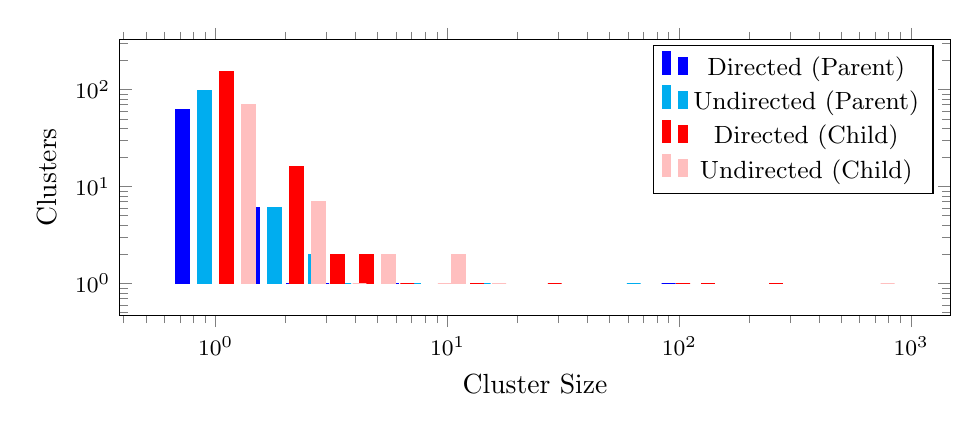
\begin{tikzpicture}
          \begin{loglogaxis}[
              height=2in,
              width=\textwidth,
              ybar=3pt,
              ylabel=Clusters,
              xlabel=Cluster Size,
              bar width=5pt,
              enlargelimits=0.15,
              legend entries={Directed (Parent), Undirected (Parent), Directed (Child), Undirected (Child)}
            ]
            \addplot[draw=blue, fill=blue]
            coordinates { (1,62) (125,1) (2,6) (3,1) (4,1) (8,1) };
            \addplot[draw=cyan, fill=cyan]
            coordinates { (1,97) (16,1) (2,6) (3,2) (4,1) (71,1) (8,1) };
            \addplot[draw=red, fill=red]
            coordinates { (1,154) (119,1) (12,1) (2,16) (234,1) (26,1) (3,2) (4,2) (6,1) (9,1) (93,1) };
            \addplot[draw=pink, fill=pink]
            coordinates { (1,70) (12,1) (2,7) (3,1) (4,2) (569,1) (7,1) (8,2) };
          \end{loglogaxis}
        \end{tikzpicture}
        \caption{MMHF Cluster Counts}
        \label{fig:mmhfhist}
      \end{figure}

      Sample execution timings of the most time-intensive functions for a MMHF parent process and child are given in Table~\ref{tbl:mmhftp}
      and Table~\ref{tbl:mmhftc}, respectively. A few exceptions denote
      TURTLES procs and functions whose names forced a refactoring of the proc name sanity check.


      \paragraph{}{
        {\footnotesize
          \begin{longtable}{l r r r}
            \toprule
            Callee & Calls & $t_{total}$ ($\mu$s) & $t_{avg}$ ($\mu$s) \\
            \midrule \\
            \endhead \\
            ::turtles::on\_proc\_enter & 58214 & 3264605 & 56 \\
            ::turtles::on\_proc\_leave & 58208 & 3228439 & 55 \\
            ::radarbox & 44354 & 1150864 & 25 \\
            ::feedstream::initialize & 1 & 1038205 & 1038205 \\
            ::feedstream::reload\_airport\_aliases\_and\_airline\_codes & 1 & 1014875 & 1014875 \\
            ::tcl::clock::format & 990 & 496919 & 501 \\
            ::tcl::clock::ParseClockFormatFormat & 54 & 326480 & 6045 \\
            ::tcl::clock::ParseClockFormatFormat2 & 54 & 265048 & 4908 \\
            ::tcl::clock::LocalizeFormat & 54 & 211535 & 3917 \\
            ::msgcat::mc & 648 & 167107 & 257 \\
            ::fa\_def\_facility & 4316 & 105557 & 24 \\
            ::fa\_cat::setcat & 3004 & 77515 & 25 \\
            ::load\_airline\_statics & 1 & 54691 & 54691 \\
            ::sqlbird::select & 1 & 54440 & 54440 \\
            \vdots & \vdots & \vdots & \vdots \\
            ::turtles::persistence::base::finalize & 1 & 17874 & 17874 \\
            ::tcl::clock::formatproc'\%B'cs\_cz & 24 & 694 & 28 \\
            ::tcl::clock::formatproc'\%a \%b \%d \%H:\%M:\%S \%Z \%Y'c & 1 & 103 & 103 \\
            \vdots & \vdots & \vdots & \vdots \\
            \bottomrule \\
            \caption{MMHF Parent Execution Timings}
            \label{tbl:mmhftp}
        \end{longtable}}
      }
      \paragraph{}{
        {\footnotesize
          \begin{longtable}{l r r r}
            \toprule
            Callee & Calls & $t_{total}$ ($\mu$s) & $t_{avg}$ ($\mu$s) \\
            \midrule \\
            \endhead \\
            ::consume\_rmq & 142 & 30512117 & 214874 \\
            ::process\_parsed\_line & 142 & 30440310 & 214368 \\
            ::really\_process\_parsed\_line & 142 & 29504325 & 207776 \\
            ::supercatch & 142 & 26035885 & 183351 \\
            ::handle\_position & 73 & 24797668 & 339694 \\
            ::handle\_position\_after\_tita\_check & 69 & 23757255 & 344308 \\
            ::handle\_vetted\_position & 69 & 23713692 & 343676 \\
            ::process\_position\_for\_all\_pedigreed\_forks & 67 & 20238384 & 302065 \\
            ::handle\_asdi\_adsb & 52 & 20047812 & 385534 \\
            ::process\_position\_for\_one\_fork & 211 & 19930730 & 94458 \\
            ::turtles::on\_proc\_leave & 141295 & 14090878 & 99 \\
            ::turtles::on\_proc\_enter & 141303 & 13940794 & 98 \\
            \vdots & \vdots & \vdots & \vdots \\
            \bottomrule
            \caption{MMHF Child Execution Timings}
            \label{tbl:mmhftc}
        \end{longtable}}
      }
      The count of unused procs for this parent process came to 6324. By contrast, a sample child process reported 5581 unused procs.
      The discrepancy is likely composed of the functions which the children use to perform the actual message processing whereas
      the parent simply manages the children.
    }
  }
}
\section{Conclusions}{
  A number of challenges were encountered during the course of development, many of which arose from the author's unfamiliarity
  with the Tcl language.

  The complete isolation of threads into separate Tcl interpreters was a boon for reasoning about safety and contention since
  there could be no bleed between threads except as explicitly delivered by message or thread state variable. Conversely,
  it was not immediately obvious that all the prior package and source imports done in the main thread needed to be replicated
  for every \texttt{thread::create}. Some reduction of this obligatory boilerplate, perhaps as an option passed to
  \texttt{thread::create} to copy imports to the spawned thread, would be welcome. Equally not obvious was whether trace
  handlers would survive a fork boundary crossing, but these thankfully persisted. Otherwise, the fork safety mechanism would
  require a substantial increase in complexity to be of use.

  The inconsistent behavior of forking across platforms was also an impediment. The fork safety mechanisms were tested on FreeBSD
  and Linux, but the support for forking in Tcl on MacOS X has at least one outstanding issue that has remained open for years\autocite{c4e230f29b}.
  The age of this bug and Apple's inexorable march toward locking down development on MacOS X (cf. the release notes for Catalina\autocite{scriptsonmac})
  leave little hope for improvement in this regard. Consequently, the forking cases are skipped when building
  and installing on MacOS X, and users of TURTLES should take this into consideration during development.
  
  Attempting to leverage signal trapping
  in multithreaded code raised similar issues\autocite{bounty32} when trying to instrument programs like Slowbird.
  There appears to be critical technical debt left outstanding with respect to Tcl's interfacing with the various operating systems
  on which it is available.

  As a relative newcomer to the language, trying to keep straight the levels of string escaping and avoiding over-substitution
  proved difficult, especially as it related to passing thread messages. The thread message passing model itself incurs significant
  overhead, and there are likely better ways to deliver call record updates to the recorder thread.

  The TURTLES project made extensive use of Tcl dictionaries as they were easier to manipulate than Tcl arrays. Frequently,
  the data layout encouraged the nesting of dictionaries which is reasonable in theory but suboptimal in practice. Making minor
  adjustments to deep layers in a nested dictionary proved slow, and the syntactically elegant \texttt{dict with} subcommand
  often had to be eschewed for more verbose forms to access and update dictionary contents. The most salient example of this
  was the apparent inability to add keys at the deepest level of a \texttt{dict with} body since variable assignments to
  heretofore unknown variable names are placed in the global namespace when unqualified. The lack of an intelligent, generic dictionary
  comparator also hampered efforts to quickly construct unit tests since Everything Is A String (EIAS).

  The interaction between \texttt{info}, \texttt{uplevel}, and \texttt{namespace} could stand to be comprehensively documented
  with representative examples. It was not until late in the development cycle that \texttt{namespace origin} supplanted \texttt{namespace which}
  so that aliased calls could be properly associated with their respective definitions and thus produce more accurate call graphs.

  With all that said, developing the TURTLES library served as an informative immersion into Tcl and its paradigms. The several outstanding
  issues that were encountered are not insoluble but do require some targeted attention to help Tcl improve as a platform for development.
  The TURTLES library appears to have achieved most of its goals apart from performance and support for certain execution edge cases.
  Some of the areas for potential improvement of the TURTLES library are expounded upon in the following Future Work section.
}

\section{Future Work}{
  As stated previously, the performance of TURTLES leaves something to be desired. Smoke tests with Slowbird exhibited a slowdown
  in execution under instrumentation by about half. To this end, a restructuring of the communication with the recorder thread
  is proposed. By using chans and designing a simple protocol, the need for complex snippets can be obviated, and the messages
  can be reduced appropriately to mere data. Some work is required to determine whether this is feasible, but it seems like the
  simplest solution with the highest potential for gain.

  While persisting to SQLite is sufficient for singly executing programs, the demands of multiple workers may necessitate a
  more scalable persistence mechanism. The obvious choice is a PostGreSQL database, to which much of the logic already present
  could be easily ported. This would also enable quicker aggregation over multiple runs if each run included a run ID as a column
  in a set of multi-run tables.

  The TURTLES project has so far focused exclusively on proc tracing. Adding variable tracing would boost the usefulness of the
  project since records of variable access can provide another window into code patterns (or anti-patterns) and memory usage.

  The issue of trace ID determinism has been resolved for the current scope and implementation. However, it would be beneficial
  if there were a descent path ID that traced an execution path from root call to leaf in order to provide more granular call graphs
  with greater confidence. This may require modification of the Tcl interpreter itself to ensure consistency and correctness.

  One last avenue of future development is to research retroactive and automatic instrumentation. It may not always
  be possible to bootstrap the TURTLES library early enough, or it may be desired to attach to a running Tcl program and
  turn instrumentation on and off at will. Being able to retroactively load trace handlers for
  existing commands and to transparently load instrumentation during thread spawns would complete the execution picture.

  The TURTLES project has been demonstrated to successfully trace and report execution behavior of different types of programs,
  even across fork boundaries. While there is a rich and daunting field of future work to pursue, the author hopes that this
  effort will contribute to improving the Tcl platform for neophytes and veterans alike.
}

\printbibliography

\end{document}
